\documentclass[
  aps,
  prd,
  preprint,
  nofootinbib,
  superscriptaddress,
  longbibliography
]{revtex4-2}

\usepackage{amsmath,amssymb,amsfonts}
\usepackage{bm}
\usepackage{array}
\usepackage{booktabs}
\usepackage{tikz}
\usepackage{placeins}
\usepackage[hidelinks]{hyperref}
\usetikzlibrary{arrows.meta,positioning,shapes.geometric}

\newcommand{\Spin}{\mathrm{Spin}}
\newcommand{\SO}{\mathrm{SO}}
\newcommand{\SU}{\mathrm{SU}}
\newcommand{\U}{\mathrm{U}}
\newcommand{\CP}{\mathbb{CP}}
\newcommand{\cO}{\mathcal{O}}
\newcommand{\GeV}{\mathrm{GeV}}
\newcommand{\aut}{\mathfrak{aut}}
\newcommand{\sltwo}{\mathfrak{sl}_2(\mathbb C)}
\DeclareMathOperator{\Tr}{Tr}
\DeclareMathOperator{\Res}{Res}
\DeclareMathOperator{\ad}{ad}
\DeclareMathOperator{\divisor}{div}

\newtheorem{theorem}{Theorem}[section]
\newtheorem{proposition}[theorem]{Proposition}
\newtheorem{lemma}[theorem]{Lemma}
\newtheorem{corollary}[theorem]{Corollary}
\newtheorem{definition}[theorem]{Definition}
\newtheorem{assumption}[theorem]{Assumption}
\newtheorem{principle}[theorem]{Principle}
\newtheorem{anchor}[theorem]{Empirical Anchor}
\newtheorem{datum}[theorem]{Benchmark Datum}
\newtheorem{observation}[theorem]{Observation}
\newtheorem{remark}[theorem]{Remark}
\newenvironment{proof}{\par\noindent\textit{Proof.}\ }{\hfill\(\square\)\par}

\begin{document}

\title{\texorpdfstring{A First-Principles Reconstruction of the
Face-Projection \(\Spin(10)\) Framework:\\
Enumerated Six-Face Uniqueness, Automorphism-Protected Families,
the Killing Contact, and the Provable Conditional Boundary}
{A First-Principles Reconstruction of the Face-Projection Spin(10)
Framework}}
\author{BoYu Chen}
\email{boypatrick.tw@gmail.com}
\affiliation{Independent Researcher, Hsinchu, Taiwan}
\date{July 4, 2026}

\begin{abstract}
This note rewrites the companion lean face-projection note as a derivation
from four explicitly stated principles: consistency (anomaly-free
four-dimensional chiral gauge theory), face projection (the visible labels
are the restriction of one complex irreducible representation of one compact
simple group), a self-carried index (the protected family space is the
automorphism algebra of the family curve), and a canonical contact (the
Majorana contact is algebra-derived and nondegenerate).  Relative to the
companion note, four items move from conditional inputs or remarks to
theorems.  First, an exact enumeration over every simple algebra of rank
4--15 plus the exceptional groups shows that no fifteen-dimensional
single-object realization of one Standard-Model family exists and that at
dimension sixteen the \(\Spin(10)\) half-spinor is the unique anomaly-free
realization; the sixteenth state \(\nu^c\) is therefore forced, not assumed.
Second, the genus ladder \(h^0(\Sigma_g,T_{\Sigma_g})=3,1,0\) makes three
families an a-priori maximum; the Cartan criterion selects \(g=0\), so the
rational family curve, the \(\cO(2)\) carrier, exactly three families, and
the two-center divisor---the Poincar\'e--Hopf zero divisor of a Cartan
flow---are derived rather than chosen.  Third, the contact direction equals
the Killing form of the family algebra, \(B=2\sqrt3\,K_{\rm tr}\), so its
existence and nondegeneracy follow from the same simplicity that fixes the
family number.  Fourth, the hidden-messenger superpotential of the
companion note's optional extension is form-unique, leaving a single complex
coupling with \(\lambda^2=\zeta\).  A closing boundary theorem proves, by a
two-model argument with an internal witness family (the same messenger
theory at variable coupling), that no value of \(\zeta\) is a consequence of
any such principle set: the companion note's boxed corollary is thereby
upgraded from a claim boundary to a theorem.  Every arithmetic and
linear-algebra step is reproduced by two machine audits (44 + 24 checks);
the second closes the former classical-input citations by direct
computation, including the longest-Weyl-element classification of complex
representations and the exactly vanishing cubic anomaly tensor of the
\(16\) built from five fermionic modes.  String-theoretic readings enter
only as optional interpretations.  This note adds no phenomenology; the
companion note's deferred audits are unchanged.
\end{abstract}

\maketitle

\section{Scope and Relation to the Companion Note}
\label{sec:scope}

The companion lean note\footnote{\texttt{paper/gut\_framework.tex} in the
same repository; cited below as ``the companion note.''} establishes a
bounded theorem stack---the six-face \(\Spin(10)\) skeleton, the
\(\Spin^c(\CP^1,\cO(2))\) family index, and the unique transvectant contact
direction \(K_{\rm tr}\)---and then deliberately stops, recording everything
else as conditional inputs, deferred audits, or optional interpretations.
Its central boxed statement is that face-projection motivation plus a
conditional \(\Spin(10)\) effective theory is \emph{not} an unconditional
principles-only proof of a grand unified theory.

This note asks the converse question: given that boundary, how much of the
skeleton and of the conditional-input list can be derived from a small,
explicitly stated principle set---and can the residue be proven
irreducible?  The answer, developed below, is:

\begin{enumerate}
\item the six-face object, including the sixteenth state \(\nu^c\), the
  hypercharge normalization \(k_Y=5/3\), and the uniqueness of the
  \(\Spin(10)\) half-spinor, follows from the consistency and
  face-projection principles by exact enumeration (Sec.~\ref{sec:sixface});
\item the rational family curve, the \(\cO(2)\) carrier, the two-center
  divisor, and the family number \(N_{\rm fam}=3\) follow from the
  self-carried-index and canonical-contact principles, with
  \(N_{\rm fam}\le3\) as an a-priori bound (Sec.~\ref{sec:families});
\item the contact direction is the Killing form of the family algebra, with
  existence, nondegeneracy, and uniqueness all consequences of simplicity
  (Sec.~\ref{sec:killing});
\item the hidden-messenger superpotential is form-unique with a single
  residual complex coupling (Sec.~\ref{sec:messenger});
\item no value of that coupling---equivalently of \(\zeta\)---is a
  consequence of the principles: the companion note's conditional boundary
  is itself a theorem (Sec.~\ref{sec:boundary}).
\end{enumerate}

This note does not modify the companion note.  It is a candidate
restatement, kept in its own directory under the repository's promotion
discipline: the companion note's ledger is relocated only if this
reconstruction is accepted.  Two machine audits replay every step (44 + 24
checks) and write ledgers with explicit negative-boundary flags
(Sec.~\ref{sec:manifest}); the provenance ledger of
Sec.~\ref{sec:provenance} classifies every external ingredient as
machine-verified, textbook-cited, retained input, or benchmark
corroboration.  The companion note's formerly deferred flavor,
proton-decay, threshold, and source-sector audits have since been
executed as standalone machine-checked scripts;
Sec.~\ref{sec:falsifiability} collects their outcome as a branch map and
an explicit list of kill criteria, each tagged with the branch it
falsifies.

\begin{remark}[Repository terminology]
\label{rem:terminology}
In the project repository, the companion lean note, its optional
hidden-messenger extension, its optional string-constrained interpretation,
and the present reconstruction are filed under the working aliases
``route~A,'' ``route~B,'' ``route~D,'' and ``route~E,'' respectively.
The dynamics-audit ledgers cited in Sec.~\ref{sec:falsifiability} are
filed under working aliases ``DYN-0''--``DYN-9,'' and the three
string-conditional pricing cards under ``D3''--``D5.''  All of these
aliases are file-system labels, not scientific claims; outside this
remark and the literal file paths in
Secs.~\ref{sec:falsifiability}--\ref{sec:manifest} they do not occur in
this paper.
\end{remark}

\subsection{Relation to prior work}
\label{sec:prior}

The ingredients have long histories, which the provenance ledger keeps
separate from the new assembly.  The \(\Spin(10)\) family spinor and its
binary/oscillator reading go back to
Refs.~\cite{Georgi1975,FritzschMinkowski1975}, with a modern mathematical
exposition in Ref.~\cite{BaezHuerta2010}; anomaly safety of the orthogonal
series is classical \cite{GeorgiGlashow1972,Okubo1977}, and the relevant
global anomaly vanishes because \(\pi_4(\Spin(10))=0\)
\cite{WittenSU2Anomaly1982}.  The index-protection idea descends from the
paradigm that the generation number is a compactification index
\cite{CandelasHorowitzStromingerWitten1985}.  The family-symmetry tradition
ordinarily imposes a continuous or discrete family group externally
\cite{KingLuhn2013}.  The present reconstruction differs at three points,
which we have not found combined in the literature: the family space is
required to be the automorphism algebra of its own carrier (the covariance
group is generated, not imposed); the family number is then bounded a
priori by three, with equality forced by the Cartan criterion; and the
Majorana contact direction is the Killing form of that algebra.  These are
claimed as new assemblies of standard mathematics, not as new mathematics.

\section{The Principle Set and the Anchors}
\label{sec:principles}

All derivations below are unconditional \emph{relative to the following
principles}.  The principles themselves are inputs; the point of this note
is to make the input list minimal and explicit, and then to prove
(Sec.~\ref{sec:boundary}) that the remaining conditional residue cannot be
absorbed into any principle set of this kind.

\begin{principle}[Consistency]
\label{pr:consistency}
The low-energy theory is a four-dimensional chiral gauge theory; all gauge
anomalies of the high-energy gauge group must cancel within the posited
chiral matter content.
\end{principle}

\begin{principle}[Face projection]
\label{pr:face}
Visible multiplet labels are not primitive.  They are the irreducible
summands of the restriction
\(\Pi_\theta(R)=\Res^{G}_{H_\theta}R\)
of a \emph{single} complex irreducible representation \(R\) of a
\emph{single} compact simple group \(G\) to the Standard-Model face
\(H_\theta\simeq\SU(3)_C\times\SU(2)_L\times\U(1)_Y\)
\cite{PatiSalam1974,Georgi1975,FritzschMinkowski1975,Slansky1981}.
\end{principle}

\begin{principle}[Self-carried index]
\label{pr:index}
The family multiplicity is the dimension of a protected zero-mode space of
an elliptic operator on a compact internal family curve \(\Sigma\), not a
tunable integer; all other SM-charged internal sectors are absent, gapped,
or vectorlike.  In addition---the strengthening introduced here---the
family carrier introduces no auxiliary data: it is the holomorphic tangent
bundle of the family curve itself, so that the protected family space
\emph{is} the automorphism algebra of the family geometry,
\[
  V=H^0(\Sigma,T_\Sigma)=\aut(\Sigma).
\]
\end{principle}

\begin{principle}[Canonical contact]
\label{pr:contact}
The Majorana contact tensor is not adjustable data: it must be a
nondegenerate invariant symmetric bilinear form on \(V\) determined
canonically by the family geometry itself, with no externally chosen
tensor.
\end{principle}

Two empirical anchors state what the theory is a theory of; they are shared
by every model considered in this note.

\begin{anchor}[Observed content]
\label{an:content}
The Standard-Model face displays exactly the fifteen chiral Weyl states of
one family, \(Q,\,L,\,u^c,\,d^c,\,e^c\) with their standard quantum
numbers, possibly together with finitely many total SM singlets, and no
exotics.
\end{anchor}

\begin{anchor}[Existence]
\label{an:exist}
At least one family exists.
\end{anchor}

Note what is \emph{not} anchored: the family number three is not assumed
anywhere below---it is derived in Sec.~\ref{sec:families}---and no property
of \(\zeta\) is anchored beyond its existence as a coefficient.

\begin{figure}[!htbp]
\centering
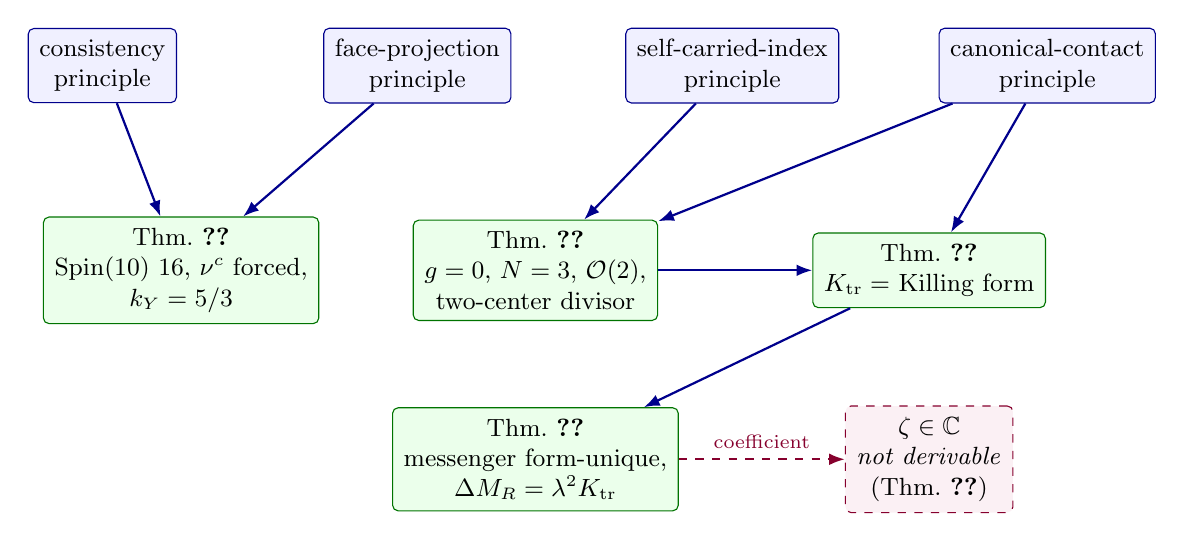
\begin{tikzpicture}[
  every node/.style={font=\small},
  box/.style={draw=blue!55!black, rounded corners=2pt, fill=blue!6,
    inner sep=4pt, align=center},
  thm/.style={draw=green!45!black, rounded corners=2pt, fill=green!8,
    inner sep=4pt, align=center},
  bad/.style={draw=purple!70!black, rounded corners=2pt, fill=purple!6,
    inner sep=4pt, align=center, dashed},
  arr/.style={-{Latex[length=2mm]}, blue!55!black, thick}
]
\node[box] (pcons) at (-6.0,2.6) {consistency\\principle};
\node[box] (pface) at (-2.0,2.6) {face-projection\\principle};
\node[box] (pidx) at (2.0,2.6) {self-carried-index\\principle};
\node[box] (pcont) at (6.0,2.6) {canonical-contact\\principle};
\node[thm] (t1) at (-5.0,0.0) {Thm.~\ref{thm:sixface}\\ \(\Spin(10)\) 16,
  \(\nu^c\) forced,\\ \(k_Y=5/3\)};
\node[thm] (t2) at (-0.5,0.0) {Thm.~\ref{thm:threefam}\\ \(g=0\), \(N=3\),
  \(\cO(2)\),\\ two-center divisor};
\node[thm] (t3) at (4.5,0.0) {Thm.~\ref{thm:killing}\\
  \(K_{\rm tr}=\) Killing form};
\node[thm] (t4) at (-0.5,-2.4) {Thm.~\ref{thm:messenger}\\ messenger
  form-unique,\\ \(\Delta M_R=\lambda^2K_{\rm tr}\)};
\node[bad] (z) at (4.5,-2.4) {\(\zeta\in\mathbb C\)\\ \emph{not derivable}\\
  (Thm.~\ref{thm:boundary})};
\draw[arr] (pcons) -- (t1);
\draw[arr] (pface) -- (t1);
\draw[arr] (pidx) -- (t2);
\draw[arr] (pcont) -- (t2);
\draw[arr] (pcont) -- (t3);
\draw[arr] (t2) -- (t3);
\draw[arr] (t3) -- (t4);
\draw[arr, dashed, purple!70!black] (t4) -- (z)
  node[midway, above, purple!70!black] {\scriptsize coefficient};
\end{tikzpicture}
\caption{Logical dependency of the reconstruction.  Solid arrows are
theorems; the dashed edge marks the unique point where a continuous datum
enters, and Theorem~\ref{thm:boundary} proves that no principle set of this
kind can supply it.}
\label{fig:dependency}
\end{figure}

\subsection{Provenance and dependency ledger}
\label{sec:provenance}

Every external ingredient of this note falls into exactly one of four
classes; nothing below is used outside its class.

\begin{description}
\item[Machine-verified here (dependency-closure audit, 24 checks).]
The conjugation involutions \(-w_0\) for every simple algebra of rank
\(4\)--\(15\) and \(E_6,E_7,E_8,F_4\); the nonzero \(\SU(15)/\SU(16)\)
fundamental cubic traces; the exactly vanishing cubic anomaly tensor of the
\(\Spin(10)\) \(16\), built from five fermionic modes, over all \(45^3\)
generator triples, with its Cartan weights reproducing the demicube; the
exceptional minima \(27,56,26,248\) and the rank-16 smallest dimensions
\(17,33,32,32\).  These are the four computations listed as (i)--(iv) in
Sec.~\ref{sec:sixface}.
\item[Machine-verified here (first-principles audit, 44 checks).]
The demicube face content and \(k_Y=5/3\); the dimension-\(\le16\)
enumeration; the genus ladder; the one-dimensionality of the invariant
contact and the identity \(B=2\sqrt3\,K_{\rm tr}\); the Schur complement;
the \(\zeta\)-independence witness.
\item[Textbook theorems (cited with statements, not rederived).]
The Weyl dimension formula and highest-weight theory
\cite{FultonHarris1991}; Riemann--Roch and Serre duality
\cite{GriffithsHarris1978}; the Cartan criterion \cite{FultonHarris1991};
the identification of a section's zero divisor with \(c_1\)
(Poincar\'e--Hopf) \cite{GriffithsHarris1978}; the Dolbeault--Hodge
identification \cite{LawsonMichelsohn1989}; \(\pi_4(\Spin(10))=0\)
\cite{WittenSU2Anomaly1982}; minimal-dimension tables for rank
\(\ge17\) \cite{Slansky1981}.
\item[Retained inputs (axioms and matching-level choices).]
(i)~the four principles; (ii)~the two empirical anchors; (iii)~the
minimal-dimension tie-break in Theorem~\ref{thm:sixface} (an Occam clause;
dropping it reopens, e.g., the \(E_6\) \(27\) with vectorlike extra
matter); (iv)~the \(U(1)_R\) charge assignment of the hidden-messenger
sector --- the Majorana-only selection rule is \emph{derived} from it in
the companion note, but the assignment itself is an input; (v)~the
post-\(B\!-\!L\) projector \(P_{\nu^c}\); (vi)~\(\mu\ne0\) and the
no-extra-unpaired-sector clause of the self-carried-index principle.
\item[Companion-note benchmark data (corroboration only, never premises).]
The \(\zeta\) digits, the sensitivity windows, the \(\mathbb Z_{N\le6}\)
miss, the \(N=178\) diagnostic, and the phase-transfer invariants.  They
illustrate Theorem~\ref{thm:boundary}; no theorem in this note has them
among its hypotheses.
\end{description}

After Sec.~\ref{sec:boundary} replaces the witness family by the internal
hidden-messenger family, this note has \emph{no} dependency on the
repository's string-constrained sandbox: the local F-theory and instanton
readings are cited only as optional UV interpretations.  The item-by-item
status of this closure is tracked in the roadmap file listed in
Sec.~\ref{sec:manifest}.

\section{Six Faces from Enumeration}
\label{sec:sixface}

The companion note states the six-face proposition as a ``standard
minimal'' realization.  This section upgrades it to an enumerated
uniqueness theorem and shows that the sixteenth state is a prediction.

\begin{lemma}[Chirality forces complexity]
\label{lem:complex}
If \(\Res^G_{G_{\rm SM}}R\) satisfies the observed-content anchor, then
\(R\) is a complex representation of \(G\).
\end{lemma}

\begin{proof}
Restriction commutes with complex conjugation, so the restriction of a
self-conjugate representation is self-conjugate.  The anchored content is
not self-conjugate as a \(G_{\rm SM}\) representation: its hypercharge
multiset contains \(Y=1/6\) with multiplicity six but \(Y=-1/6\) with
multiplicity zero, and the possible extra SM singlets are self-conjugate,
so they cannot repair the mismatch.  Hence \(R\) cannot be real or
pseudoreal.
\end{proof}

\begin{lemma}[Rank bound]
\label{lem:rank}
\(G\supseteq G_{\rm SM}\) implies \(\mathrm{rank}\,G\ge4\).
\end{lemma}

\begin{proof}
A maximal torus of \(G_{\rm SM}\), of dimension four, embeds in a maximal
torus of \(G\).
\end{proof}

The classification formerly rested on four classical inputs.  All four are
now machine-verified by the dependency-closure audit and enter as checked
computations, with the textbook context retained as background
\cite{Slansky1981,Georgi1975,FultonHarris1991,GeorgiGlashow1972,Okubo1977}:
\begin{itemize}
\item[(i)] the conjugation involution \(-w_0\), computed from the Cartan
  matrix by \(\rho\)-descent for every simple algebra of rank \(4\)--\(15\)
  and for \(E_6,E_7,E_8,F_4\), is the label reversal for \(A_n\), the
  spinor-node swap for \(D_{2k+1}\), the arm flip for \(E_6\), and the
  identity (\(w_0=-1\)) for \(B_n\), \(C_n\), \(D_{2k}\), \(E_7\), \(E_8\),
  \(F_4\); hence only \(A_n\), \(D_{2k+1}\), \(E_6\) admit complex
  irreducibles;
\item[(ii)] a single Weyl fermion in the fundamental of \(\SU(15)\) or
  \(\SU(16)\) is gauge-anomalous: on an exact integer diagonal generator,
  \(\Tr T^3=2730\) and \(3360\), respectively
  \cite{GeorgiGlashow1972,Okubo1977};
\item[(iii)] the chiral \(16\) of \(\Spin(10)\), constructed explicitly
  from five fermionic modes (chirality \(=\) occupation parity), satisfies
  \(\Tr(\{T_a,T_b\}T_c)=0\) exactly over all \(45^3\) generator triples,
  and its Cartan weights reproduce the demicube of
  Appendix~\ref{app:demicube}; the nonperturbative check,
  \(\pi_4(\Spin(10))=0\), remains cited rather than computed
  \cite{WittenSU2Anomaly1982};
\item[(iv)] the exceptional minima are \(27\) (\(E_6\)), \(56\) (\(E_7\)),
  \(26\) (\(F_4\)), \(248\) (\(E_8\)) by direct scan, so no exceptional
  group contributes at dimension \(\le16\).
\end{itemize}

\begin{lemma}[Monotonicity of the Weyl dimension]
\label{lem:monotone}
For a fixed simple algebra, the Weyl dimension
\(\dim\lambda=\prod_{\alpha>0}\langle\lambda+\rho,\alpha^\vee\rangle/
\langle\rho,\alpha^\vee\rangle\)
is strictly increasing in each Dynkin label.
\end{lemma}

\begin{proof}
Each factor is a positive linear form in the labels with nonnegative
coefficients divided by a positive constant, and every label appears with a
positive coefficient in at least one factor (e.g.\ the corresponding simple
root).
\end{proof}

Lemma~\ref{lem:monotone} makes the following finite search exhaustive; it
is performed with exact rational arithmetic in the machine audits.

\begin{proposition}[Enumeration at dimension \(\le16\)]
\label{prop:enumeration}
Among all simple compact groups of rank \(\ge4\) --- every algebra of rank
\(4\)--\(15\) (\(A_n\), \(B_n\), \(C_n\), \(D_n\), \(E_6\), \(E_7\),
\(E_8\), \(F_4\)) is scanned directly, while rank \(\ge16\) contributes
nothing because the smallest rank-16 irreducibles already have dimensions
\(17,33,32,32\) (machine-checked) and the corresponding minima grow with
rank (minimality per the tables of Ref.~\cite{Slansky1981}, cited) --- the
complete list of complex irreducible representations of dimension \(15\) or
\(16\) is:
\[
\begin{array}{c|c|c}
\dim & \text{representation} & \text{fate}\\
\hline
15 & \SU(5):\ \mathrm{Sym}^2\,5 & \text{color sextet (Lemma~\ref{lem:content15})}\\
15 & \SU(6):\ \Lambda^2\,6 & \text{content fails (Lemma~\ref{lem:content15})}\\
15 & \SU(15):\ \text{fund.} & \text{anomalous, item (ii)}\\
16 & \SU(16):\ \text{fund.} & \text{anomalous, item (ii)}\\
16 & \Spin(10):\ 16 & \text{survives}
\end{array}
\]
together with the conjugates of each entry.
\end{proposition}

\begin{remark}[Self-conjugate near-misses]
\label{rem:nearmiss}
The same scan returns two instructive non-complex entries at these
dimensions: \(\mathfrak{so}(9)\) possesses a \emph{real} spinor of
dimension exactly \(16\), and \(\mathfrak{so}(15)\) a real vector of
dimension \(15\).  Both fail Lemma~\ref{lem:complex}, not the dimension
count.  Complexity --- that is, chirality --- and not size alone is what
selects \(\Spin(10)\).
\end{remark}

\begin{lemma}[Content eliminations at dimension 15]
\label{lem:content15}
No embedding \(G_{\rm SM}\subset\SU(5)\) or \(G_{\rm SM}\subset\SU(6)\)
makes \(\mathrm{Sym}^2\,5\) or \(\Lambda^2\,6\) satisfy the
observed-content anchor.
\end{lemma}

\begin{proof}
\(\SU(5)\): if the restriction of the \(5\) contains no color triplet, the
restriction of \(\mathrm{Sym}^2 5\) contains no quarks and the anchor
fails.  If it contains a triplet, then
\(\mathrm{Sym}^2 5\supset\mathrm{Sym}^2(3,\cdot)=(6,\cdot)\), a color
sextet, which is an exotic.

\(\SU(6)\): decompose the \(6\) under \(\SU(3)_C\times\SU(2)_L\).  If
\(6=(3,2)\), then \(\Lambda^2 6=(\bar3,3)\oplus(6,1)\) contains a sextet.
If \(6\supset(3,1)\oplus(\bar3,1)\), then
\(\Lambda^2 6\supset 3\otimes\bar3\supset(8,1)\), a color octet.  If
\(6=(3,1)\oplus(1,2)\oplus(1,1)\), then
\[
  \Lambda^2 6=(\bar3,1)\oplus(3,2)\oplus(3,1)\oplus(1,1)\oplus(1,2),
\]
which contains a single \(\bar3\) and an extra \((3,1)\); one family needs
two color antitriplets (\(u^c,d^c\)) and no \((3,1)\), so the anchor fails.
If the \(6\) contains two triplets, \(3\otimes3\supset(6,1)\) appears.  No
case survives.
\end{proof}

\begin{theorem}[Enumerated six-face uniqueness]
\label{thm:sixface}
Under the consistency and face-projection principles and the
observed-content anchor, the minimal-dimension realization exists, is
unique, and is the \(\Spin(10)\) half-spinor \(16\).  Its Standard-Model
face is exactly
\[
  \Res^{\Spin(10)}_{G_{\rm SM}}16
  =Q\oplus L\oplus u^c\oplus d^c\oplus\nu^c\oplus e^c ,
\]
with multiplicities \((6,2,3,3,1,1)\) as Weyl states.
\end{theorem}

\begin{proof}
By Lemma~\ref{lem:complex} the representation is complex; by
Lemma~\ref{lem:rank} the group has rank \(\ge4\), and by the computed
involutions (item (i)) the complex candidates within the scan range are the
\(A_n\), \(D_{2k+1}\), \(E_6\) families.  By the observed-content anchor
the dimension is \(15\) plus the number of SM singlets, so the minimal
candidates have dimension \(15\) or \(16\).
Proposition~\ref{prop:enumeration}, Lemma~\ref{lem:content15}, and the
exact cubic traces (item (ii)) eliminate every candidate except the
\(\Spin(10)\) half-spinor, which is anomaly-free by item (iii).  Existence
and the displayed face content are the standard Pati--Salam branching,
verified at weight level in Appendix~\ref{app:demicube}: the sixteen
even-parity \(D_5\) half-spin weights split \(8+8\) under the Pati--Salam
face and project to exactly \((Q,L,u^c,d^c,\nu^c,e^c)=(6,2,3,3,1,1)\).
\end{proof}

\begin{corollary}[The sixteenth state is a prediction]
\label{cor:nuc}
No fifteen-dimensional single-object realization of one family exists.
Under the consistency and face-projection principles the sixteenth
state---a total SM singlet, \(\nu^c\)---is forced.  The essential seesaw
ingredient is therefore an output of the face principle, not an input.
\end{corollary}

\begin{corollary}[Hypercharge normalization]
\label{cor:ky}
On the surviving object, \(Y=T_{3R}+(B-L)/2\) and
\[
  \Tr Y^2=\frac{10}{3},\qquad \Tr T_{3L}^2=2,\qquad
  k_Y=\frac53 ,
\]
exactly as in the companion note (weight-level check in
Appendix~\ref{app:demicube}).
\end{corollary}

\begin{remark}[Face covariance in action]
The standard and flipped \(\SU(5)\times\U(1)\) identifications of the same
half-spinor produce identical multisets of SM multiplet types with the
roles of \(u^c\leftrightarrow d^c\), \(\nu^c\leftrightarrow e^c\)
exchanged.  Two legal faces of one object carry the same content; only
action-level data distinguish them.  This is precisely the face-covariance
statement of the companion note, realized inside
Theorem~\ref{thm:sixface} rather than assumed.
\end{remark}

\section{Three Families from the Automorphism Principle}
\label{sec:families}

The companion note protects three families by assuming the carrier data
\((C=\CP^1,\ R=p_++p_-,\ L_R\simeq\cO(2))\) and then applying the
\(\Spin^c\) Dolbeault index.  This section derives those data from the
self-carried-index and canonical-contact principles.  The analytic inputs
are the standard Dolbeault--Hodge identification and Riemann--Roch with
Serre duality \cite{LawsonMichelsohn1989,GriffithsHarris1978}.

\begin{lemma}[Genus ladder]
\label{lem:ladder}
For a compact Riemann surface \(\Sigma_g\),
\[
  h^0(\Sigma_g,T_{\Sigma_g})
  =\begin{cases}
    3, & g=0,\\
    1, & g=1,\\
    0, & g\ge2 .
  \end{cases}
\]
\end{lemma}

\begin{proof}
\(T_{\Sigma_g}=K_{\Sigma_g}^{-1}\) has degree \(2-2g\).  For \(g=0\),
\(T\simeq\cO(2)\): Riemann--Roch gives \(h^0-h^1=2+1=3\) and Serre duality
gives \(h^1=h^0(K\otimes T^{-1})=h^0(K^2)=h^0(\cO(-4))=0\), so \(h^0=3\).
For \(g=1\), \(T\) is trivial and \(h^0=1\).  For \(g\ge2\),
\(\deg T<0\) forces \(h^0=0\).
\end{proof}

\begin{corollary}[A-priori family bound]
\label{cor:bound}
Under the self-carried-index principle, the family number obeys
\(N_{\rm fam}\le3\), with equality if and only if the family curve is
rational.  Three families is the maximum this protection mechanism can
produce, not a coincidence within it.
\end{corollary}

\begin{lemma}[Cartan selection]
\label{lem:cartan}
Among \(g=0,1\) (the cases allowed by the existence anchor and
Lemma~\ref{lem:ladder}), only \(g=0\) satisfies the canonical-contact
principle.
\end{lemma}

\begin{proof}
For \(g=1\), \(\aut(\Sigma_1)\) is the one-dimensional abelian translation
algebra; the Killing form of an abelian Lie algebra vanishes identically
(\(\ad X=0\)), so by the Cartan criterion no canonical nondegenerate
invariant form exists on \(V\), and the canonical-contact principle fails.
For \(g=0\), \(V=\aut(\CP^1)=\sltwo\) is simple, and the Cartan criterion
guarantees that its Killing form is nondegenerate.
\end{proof}

\begin{theorem}[Three families]
\label{thm:threefam}
Under the self-carried-index and canonical-contact principles and the
existence anchor: the family curve is \(\Sigma\simeq\CP^1\); the family
space is canonically the M\"obius algebra,
\(V=H^0(\CP^1,T_{\CP^1})\simeq\sltwo\); the carrier is
\(T_{\CP^1}\simeq\cO(2)\); and
\[
  N_{\rm fam}=\dim\sltwo=3 .
\]
\end{theorem}

\begin{proof}
Lemma~\ref{lem:ladder} with the existence anchor leaves \(g\in\{0,1\}\);
Lemma~\ref{lem:cartan} leaves \(g=0\).  The rest is the \(g=0\) row of the
ladder.
\end{proof}

\begin{proposition}[The two-center divisor is Poincar\'e--Hopf]
\label{prop:ph}
Let \(X_h\in V\) be any regular semisimple element (a Cartan generator,
e.g.\ \(\xi\partial_\xi\) in an affine coordinate).  Then its zero divisor
is a sum of two distinct points,
\[
  \divisor(X_h)=p_++p_-,\qquad
  \deg\divisor(X_h)=\deg T_{\CP^1}=c_1(T)[\CP^1]=\chi(S^2)=2,
\]
and \(\cO(\divisor X_h)\simeq T_{\CP^1}\simeq\cO(2)\).  The two-center
divisor \(R=p_++p_-\) of the companion note is therefore the Euler class of
the family sphere realized by a Cartan flow, and the two ``centers'' are
the two fixed points of any M\"obius flow.
\end{proposition}

\begin{proof}
\(\xi\partial_\xi\) has a simple zero at \(\xi=0\); in the coordinate
\(\eta=1/\xi\) one has \(\xi\partial_\xi=-\eta\partial_\eta\), a simple
zero at \(\eta=0\).  The zero divisor of a nonzero holomorphic section of a
line bundle on a curve represents its first Chern class, and
\(c_1(T_{S^2})[S^2]=\chi(S^2)=2\) \cite{GriffithsHarris1978}.
\end{proof}

\begin{remark}[Ledger relocation]
\label{rem:relocation2}
The companion note lists \(C=\CP^1\), \(R=p_++p_-\), and the protected
\(\Spin^c\) \(\cO(2)\) carrier as branch assumptions.  Under the
self-carried-index and canonical-contact principles all three are theorems.
What the index principle retains as an assumption is the protection clause
itself (no additional unpaired SM-charged sectors) and the self-carried
choice; the latter does real selective work, as the next remark records.
\end{remark}

\begin{remark}[Why the tangent bundle and not \(\cO(2m)\)]
For \(g=0\) one has \(h^0(K^{-m})=2m+1\), so ``some canonical bundle
power'' would allow any odd family number.  The self-carried clause is what
singles out \(m=1\): only for the tangent bundle is the family space itself
the algebra that generates the family covariance (the adjoint module),
rather than a module over an external symmetry.  Equivalently, the
\(SL(2)\) bookkeeping of the companion note stops being a spurion choice
and becomes the geometry of \(V\) acting on itself.
\end{remark}

\section{The Killing Contact}
\label{sec:killing}

The companion note proves that the invariant contact direction in
\(\mathrm{Sym}^2V^\vee\) is unique (the second transvectant) and remarks
that it resembles the Killing form.  With Theorem~\ref{thm:threefam} the
resemblance becomes an identity, and existence, nondegeneracy, and
uniqueness all follow from simplicity.

\begin{lemma}[Uniqueness]
\label{lem:unique}
\(\mathrm{Sym}^2(\mathrm{Sym}^2\mathbb C^2)
\simeq\mathrm{Sym}^4\mathbb C^2\oplus\mathrm{Sym}^0\mathbb C^2\), so the
trivial summand has multiplicity one and any invariant symmetric bilinear
form on \(V\) is unique up to scale \cite{FultonHarris1991}.  (The machine
audit verifies directly that the invariance equations
\(\rho(J)^TC+C\rho(J)=0\), \(J\in\{J_z,J_\pm\}\), have a one-dimensional
solution space.)
\end{lemma}

\begin{lemma}[Existence and nondegeneracy]
\label{lem:cartan-exist}
The Killing form \(B(x,y)=\Tr(\ad x\,\ad y)\) is an invariant symmetric
bilinear form on \(V=\sltwo\), and it is nondegenerate because \(\sltwo\)
is semisimple (Cartan criterion).
\end{lemma}

\begin{theorem}[The contact is the Killing form]
\label{thm:killing}
In the spherical orthonormal family basis
\((T_{+1},T_0,T_{-1})\) with \(T_{\pm1}=\mp J_\pm/\sqrt2\), \(T_0=J_z\),
where \(J_z,J_\pm\) are the spin-1 matrices, the Killing form of the family
algebra is
\[
  B=
  \begin{pmatrix}
    0&0&-2\\
    0&2&0\\
    -2&0&0
  \end{pmatrix}
  =2\sqrt3\,K_{\rm tr},
  \qquad
  K_{\rm tr}
  =\frac1{\sqrt3}
  \begin{pmatrix}
    0&0&-1\\
    0&1&0\\
    -1&0&0
  \end{pmatrix},
\]
including the sign pattern of the companion note's convention.
Consequently \(K_{\rm tr}^2=\tfrac13 I\) and \(K_{\rm tr}^{-1}=3K_{\rm tr}\).
\end{theorem}

\begin{proof}
The adjoint representation of \(\sltwo\) is the spin-1 representation, so
\(B(x,y)=\Tr_{3\times3}\big(R_1(x)R_1(y)\big)\) exactly.  With
\(\Tr J_z^2=2\), \(\Tr J_+J_-=4\), \(\Tr J_\pm^2=0\):
\[
  B(T_0,T_0)=2,\qquad
  B(T_{+1},T_{-1})=-\tfrac12\Tr J_+J_-=-2,\qquad
  B(T_{\pm1},T_{\pm1})=0 ,
\]
which is the displayed matrix; dividing by \(2\sqrt3\) reproduces
\(K_{\rm tr}\) with \(K_{\rm tr}^2=\tfrac13 I\).  Uniqueness up to scale is
Lemma~\ref{lem:unique}.
\end{proof}

\begin{remark}[One principle, two consequences]
\label{rem:weld}
The same simplicity that selects \(g=0\) and hence \(N_{\rm fam}=3\)
(Lemma~\ref{lem:cartan}) also guarantees that the seesaw contact direction
exists, is unique, and is invertible.  In a hypothetical \(g=1\) branch the
Majorana contact would have no canonical direction and the messenger mass
term \(K_{\rm tr}^{-1}(X,X)\) below could not even be written.  ``Exactly
three families'' and ``a working invariant seesaw contact'' are two faces
of one principle.
\end{remark}

\section{The Hidden-Messenger Mechanism: Form-Uniqueness}
\label{sec:messenger}

The companion note's optional extension posits a sterile family messenger
\(X\in V^\vee\) with a Majorana-only \(U(1)_R\) selection rule (kept here
as an EFT matching input, together with the post-\(B\!-\!L\) projector
\(N_i=P_{\nu^c}(16_i)\); both are tagged as retained inputs in
Sec.~\ref{sec:provenance}).  Given that rule, representation theory fixes
the rest.

\begin{theorem}[Form-uniqueness and Schur complement]
\label{thm:messenger}
The most general superpotential quadratic in \((N,X)\) compatible with
family covariance and the Majorana-only selection rule is
\[
  \frac{W_R}{M_*}
  =\frac12 M_V(N,N)+\lambda\,X(N)-\frac{\mu}2 K_{\rm tr}^{-1}(X,X),
\]
with \(\lambda,\mu\in\mathbb C\) and \(\mu\ne0\) required for a well-posed
messenger: the coupling term is forced to be the canonical evaluation
pairing (the invariant in \(V^\vee\otimes V\) is unique: the trace), and
the mass term is forced onto the unique invariant line of
\(\mathrm{Sym}^2V\), which is \(K_{\rm tr}^{-1}\) by
Lemma~\ref{lem:unique} and Lemma~\ref{lem:cartan-exist}.  After rescaling
\(X\) to set \(\mu=1\), integrating out \(X\) gives exactly
\[
  \frac{W_R^{\rm eff}}{M_*}
  =\frac12\big(M_V+\lambda^2K_{\rm tr}\big)(N,N),
  \qquad
  \Delta M_R/M_*=\lambda^2K_{\rm tr}.
\]
The mechanism carries exactly one residual complex number, and matching to
the benchmark requires \(\lambda^2=\zeta\).
\end{theorem}

\begin{proof}
The tensor structures are fixed by multiplicity one as stated; note that
writing the mass term at all requires \(K_{\rm tr}\) nondegenerate, i.e.\
Lemma~\ref{lem:cartan-exist}.  The \(X\) F-term gives
\(\lambda N-K_{\rm tr}^{-1}X=0\), so \(X=\lambda K_{\rm tr}N\), and
substitution yields
\(\frac12 M_V(N,N)+\lambda^2K_{\rm tr}(N,N)
-\frac12\lambda^2K_{\rm tr}(N,N)\), which is the displayed effective
superpotential.  (Replayed to \(10^{-14}\) over random matrices in the
machine audit.)
\end{proof}

\begin{datum}[Benchmark coefficient, kept as reproducibility anchor]
\label{dat:zeta}
\[
  \zeta=0.1076472949+0.0736514853\,i,
\]
\[
  \lambda=\sqrt{\zeta}=0.34502115743308964+0.10673473744038917\,i,
  \qquad
  |\lambda|=0.3611535729477664 .
\]
As in the companion note, only the first few significant figures are
physically meaningful; the digits are shared bit-identically with the
verifier scripts.  The tree-level matching-silence and
canonical-normalization caveats of the companion note apply unchanged.
\end{datum}

\section{The Boundary Theorem}
\label{sec:boundary}

Everything above is a theorem of the four principles (plus the stated EFT
inputs of Sec.~\ref{sec:messenger}).  Exactly one continuous quantity
remains: the value of \(\zeta\).  This section proves that the remainder is
not an accident of insufficient cleverness.

\begin{lemma}[Two-model lemma]
\label{lem:twomodel}
Let \(\mathcal A\) be any set of axioms and \(M_1,M_2\) two models
satisfying \(\mathcal A\) that disagree about a statement \(D\).  Then
neither \(D\) nor \(\neg D\) is a consequence of \(\mathcal A\).
\end{lemma}

\begin{proof}
A consequence of \(\mathcal A\) holds in every model of \(\mathcal A\).
\end{proof}

\begin{definition}[Admissible model class --- internal witness family]
\label{def:class}
Let
\[
  \mathfrak M=\{\,M_\lambda:\lambda\in\mathbb C^\times\,\}
\]
be the family of post-\(B\!-\!L\) effective theories of
Theorem~\ref{thm:messenger} at coupling \(\lambda\), all on the same
\(\Spin(10)\)/three-family skeleton.  Every member satisfies the
consistency principle --- the messenger \(X\) is a gauge singlet, so the
gauge-anomaly content is exactly that of the \(16_i\), which vanishes by
item (iii) of Sec.~\ref{sec:sixface} --- together with the remaining three
principles and both anchors, and realizes \(\zeta(M_\lambda)=\lambda^2\).
Hence \(\zeta\) ranges over \(S=\mathbb C^\times\).  The witness family is
internal: no string-theoretic input enters.  (The E3-instanton reading
\(\zeta_\Gamma=A_\Gamma e^{2\pi iT_\Gamma}\)
\cite{Witten1996,KatzVafa1996,BeasleyHeckmanVafa2008I} realizes the same
freedom as an axion-volume modulus; from here on it is cited only as an
optional UV interpretation, never as a premise.)
\end{definition}

\begin{lemma}[\(\zeta\)-independence of the skeleton]
\label{lem:zetaindep}
Every proof in Secs.~\ref{sec:sixface}--\ref{sec:messenger} is independent
of the numerical value of \(\zeta\): no step references it.  (The
first-principles audit witnesses this by replaying the structural checks
verbatim at a second value \(\zeta'\ne\zeta\) far outside the benchmark
windows.)
\end{lemma}

\begin{theorem}[The conditional boundary is necessary]
\label{thm:boundary}
Let \(\mathcal A\) be any axiom set all of whose axioms hold in every
member of \(\mathfrak M\) (the four principles and any \(\zeta\)-blind
strengthening).  Then for no \(\zeta_0\in S\) is the statement
\(\zeta=\zeta_0\) a consequence of \(\mathcal A\).  Consequently, fixing
\(\zeta\) requires an axiom that fails in part of \(\mathfrak M\)---that
is, new data (moduli stabilization, a hidden phase/radial sector), which is
precisely a conditional input in the sense of the companion note.
\end{theorem}

\begin{proof}
By Definition~\ref{def:class} and Lemma~\ref{lem:zetaindep}, pick
\(M_1,M_2\in\mathfrak M\) with \(\zeta(M_1)=\zeta_0\ne\zeta(M_2)\); both
satisfy \(\mathcal A\).  Apply Lemma~\ref{lem:twomodel} to
\(D:\ \zeta=\zeta_0\).
\end{proof}

\begin{corollary}[The companion note's boxed corollary, upgraded]
\label{cor:box}
Within \(\mathfrak M\),
\[
\boxed{
\begin{gathered}
\text{four principles}\ \Longrightarrow\ \text{the skeleton
(Thms.~\ref{thm:sixface}, \ref{thm:threefam}, \ref{thm:killing},
\ref{thm:messenger})},\\[2pt]
\text{four principles}\ \not\Longrightarrow\ \zeta ,
\qquad\text{hence}\qquad
\text{a principles-only unconditional GUT proof is impossible.}
\end{gathered}
}
\]
The boundary drawn by the companion note is not provisional modesty; in
this model class it is a theorem.
\end{corollary}

\begin{observation}[Finite-class corroboration from the companion note's scans]
\label{obs:scans}
The companion note's negative results are finite-class instances of
Theorem~\ref{thm:boundary}: the tested hidden \(D\)-quotients leave modulus
and phase flat; small monomial/clockwork phases with denominator \(N\le6\)
miss \(\arg\zeta\) by at least \(4.471595\times10^{-1}\ \mathrm{rad}\); the
first root of unity inside the loose window
\(5.424119\times10^{-5}\ \mathrm{rad}\) appears only at \(N=178\); and the
visible-spurion phase transfer of the companion note's finite diagnostic
has no hit.  All of these replay in the first-principles audit; per the
provenance ledger (Sec.~\ref{sec:provenance}) they are benchmark
corroboration and appear in no hypothesis.
\end{observation}

\begin{remark}[Diophantine diagnostics are not derivations]
The approximants \(17/178\), \(70/733\), \(87/911\) are ordinary
continued-fraction convergents of \(\arg\zeta/2\pi\) (verified in the
audit), with phase errors \(4.15\times10^{-5}\), \(6.68\times10^{-6}\),
\(2.73\times10^{-6}\ \mathrm{rad}\).  Such approximants exist for any real
phase; they are side diagnostics, exactly as the companion note treats
them.
\end{remark}

\begin{remark}[Scope honesty]
Theorem~\ref{thm:boundary} is relative to the stated model class.  A future
\emph{principled} stabilization axiom could fix \(\zeta\)---but by the
theorem it must exclude part of \(\mathfrak M\), so it is a new conditional
input carrying its own threshold and UV audit cost.  That is the companion
note's discipline restated as mathematics, not evaded.
\end{remark}

\section{Dynamics Audits and Falsifiability}
\label{sec:falsifiability}

The audits deferred by the companion note were executed in July 2026 as
standalone machine-checked scripts, one JSON/Markdown ledger pair per
audit, following the same discipline as the audits of
Sec.~\ref{sec:manifest} (every claim gated, every negative boundary
flagged).  A collector script,
\texttt{code/audit8\_dyn8\_falsifiability\_collection.py}, re-verifies
every number quoted in this section against its source ledger; its own
ledger is \texttt{output/audit8/dyn8\_falsifiability\_collection.json}.
Experimental statuses are as of 2026-07-05.

\subsection{Branch map}
\label{sec:branchmap}

The results split the framework into four layers with sharply different
logical statuses.

\begin{description}
\item[Kinematic core (supersymmetry-agnostic; machine-verified).]
The theorems of Secs.~\ref{sec:sixface}--\ref{sec:killing}: the
half-spinor sixteen with its forced sixteenth state, the three-family
index with the a-priori bound, and the Killing-form contact direction.
None of the dynamics results below touches this layer, and the
\(\overline{126}\)-type Majorana source direction survives in every
surviving branch.

\item[Supersymmetric minimal completion (EXCLUDED as a slice family).]
The benchmark supersymmetric completion (the
\(210+126+\overline{126}+10\) superpotential family in its
minimal-spectrum slice) is excluded by the combination of gauge
unification and proton decay: the unification-compatible vacuum
parameter forces the unification scale down to
\(\sim2\times10^{13}\,\mathrm{GeV}\), where the dimension-five
colored-triplet channel underproduces
\(\tau(p\to K^+\bar\nu)\) by \(7.7\) orders of magnitude against the
Super-Kamiokande bound; a joint rescue scan over the vacuum parameter,
the source coupling, and the supersymmetry scale finds \emph{zero}
living points, with the obstruction traced to the spectrum shape (the
threshold sums force a low unification scale, a dimension-six trap).
This excludes the \emph{slice family}, not the model class; the ledgers
record the distinction explicitly.

\item[Non-supersymmetric intermediate-scale variant (ALIVE; refit
required).]
With supersymmetry removed the dimension-five channel is structurally
absent, and two-step breaking through an intermediate gauge group
decouples the intermediate scale from the unification scale.  Of the
four canonical chains, two survive proton decay: the left-right chain
\(\SU(3)\times\SU(2)_L\times\SU(2)_R\times\U(1)_{B-L}\)
(intermediate scale \(10^{9.4}\,\mathrm{GeV}\), unification scale
\(10^{16.3}\,\mathrm{GeV}\), \(\tau(p\to e^+\pi^0)\sim10^{36}\,\)yr)
and the Pati--Salam chain \(\SU(4)\times\SU(2)_L\times\SU(2)_R\)
(the chain compatible with the companion note's \(210\) source sector;
\(\tau\simeq4.3\times10^{33}\,\)yr at one loop, within the
threshold-spread band of the current bound).  A perturbativity gate
shows that \emph{no} surviving chain can host the benchmark heavy
Majorana tower through the renormalizable source coupling
(\(f<4\pi\) fails by up to \(379\times\)): the benchmark contact card
is local to the excluded supersymmetric slice, and the
non-supersymmetric flavor refit --- including re-extraction of the
contact coefficient at the intermediate scale --- is \emph{required}
and open.  Consistently with Theorem~\ref{thm:boundary}, the contact
coefficient is an input in every branch; only its bookkeeping moves.

\item[String-conditional pricing cards (unpromoted).]
Three cards price string-motivated escapes without deriving anything:
a brane-instanton Majorana source (buys the tower \emph{scale},
zero texture compression: the instanton data equals the full
twelve-parameter Majorana data); a protection card for the hidden
messenger, whose enumeration yields an abelian no-go (any charge
bookkeeping that allows the Dirac Yukawa and the messenger portal ties
the messenger mass to the dangerous Dirac contamination), so closure
requires instanton zero-mode selectivity with a quantified gap; and a
high-scale supersymmetry-breaking bridge, alive on the left-right side
for a supersymmetry-breaking scale anywhere in
\([2\times10^{10},\,3.5\times10^{15}]\,\mathrm{GeV}\) and structurally
impossible on the Pati--Salam side.  These cards are conditional
interpretations under the promotion discipline of the companion note's
string appendix; they must not be cited as evidence.
\end{description}

\subsection{Kill criteria}
\label{sec:killbank}

Each entry names the criterion, the branch it falsifies (bracketed),
and the source ledger.

\begin{enumerate}
\item[K1.] \textbf{A fourth sequential chiral family} [kinematic core].
Falsifies the a-priori bound \(N_{\rm fam}\le3\) of
Theorem~\ref{thm:threefam}, hence the self-carried-index principle
itself.  Status: a fourth sequential family is strongly excluded by
Higgs-coupling data; the criterion stands as the core's cleanest
falsifier.  (Ledger: \texttt{route\_E/output/route\_e\_first\_principles.json}.)

\item[K2.] \textbf{Dirac neutrinos} [kinematic core's physical target].
Established Dirac nature (e.g.\ persistent absence of neutrinoless
double-beta decay together with positive evidence of lepton-number
conservation) removes the Majorana contact target of
Theorem~\ref{thm:killing}.  Contact essentiality is posterior-wide on
current oscillation data: \(P(\text{contact fraction}>0.01)=1.000\)
conditional on the benchmark Dirac kernels.
(Ledger: \texttt{output/audit1/dyn4b\_unconditional\_zeta.json}.)

\item[K3.] \textbf{Unification \(\times\) proton decay, supersymmetric
slice} [supersymmetric completion --- \emph{this criterion has fired}].
\(\tau(p\to K^+\bar\nu)\) short by \(7.7\) orders at the
unification-compatible point; zero living points in the joint rescue
scan.  (Ledgers: \texttt{output/audit2/dyn3\_proton\_d5\_kill\_criterion.json},
\texttt{output/audit3/dyn2b\_rescue\_scan.json}.)

\item[K4.] \textbf{The Pati--Salam window} [non-supersymmetric variant,
\(210\)-compatible chain].  At one loop
\(\tau(p\to e^+\pi^0)=4.3\times10^{33}\,\)yr against the current bound
\(2.4\times10^{34}\,\)yr: the chain is either already dead or sits
inside the Hyper-Kamiokande discovery window --- the sharpest
falsifiability statement this framework currently owns.
(Ledger: \texttt{output/audit9/dyn9\_nonsusy\_intermediate.json}.)

\item[K5.] \textbf{Proton-decay channel hierarchy} [non-supersymmetric
variant].  The left-right chain predicts
\(\tau(p\to e^+\pi^0)\sim10^{36}\,\)yr (above the ten-year
Hyper-Kamiokande reach; only partially probeable), and in the whole
non-supersymmetric branch the gauge dimension-six channel dominates: an
observed \(p\to K^+\bar\nu\)-dominated signal would disfavor the
branch.  (Same ledger as K4.)

\item[K6.] \textbf{Thermal leptogenesis} [supersymmetric slice;
soft criterion].  On the benchmark slice, thermal unflavored
leptogenesis fails by \(\sim1.5\) orders with the wrong central sign
(success probability \(0.4\%\); a \(\times3\)--\(10\) enhancement,
the size of flavored corrections, lifts it to \(34\)--\(45\%\)).
On the surviving non-supersymmetric branch the gravitino constraint
dissolves and the computation must be re-run after the required refit.
(Ledger: \texttt{output/audit7/dyn7\_leptogenesis\_argzeta.json}.)

\item[K7.] \textbf{Messenger canonical-normalization ceilings}
[hidden-messenger extension].  The one-loop audit proves light-sector
silence structurally (seesaw invariance under any invertible
redefinition of \(\nu^c\)) and quantifies the replay ceilings: an
\(R\)-breaking spurion of odd charge must satisfy
\(\varepsilon\lesssim4.4\times10^{-4}\) against the refreshed
contact-sensitivity windows; a microscopic completion violating the
ceiling is excluded.
(Ledger: \texttt{output/audit5/dyn5\_messenger\_one\_loop.json}.)

\item[K8.] \textbf{Heavy-neutrino/gauge-scale coexistence}
[string-conditional].  The instanton Majorana source \emph{requires}
the two heavier right-handed neutrinos to sit \emph{above} the
intermediate gauge scale (factors \(39\) and \(4.8\times10^{3}\) on the
Pati--Salam chain) --- impossible for a renormalizable perturbative
source.  Measuring an intermediate-scale gauge boson together with
heavy-neutrino masses below it falsifies the card.
(Ledger: \texttt{route\_d/output/d3\_instanton\_majorana\_pricing.json}.)

\item[K9.] \textbf{Zero-mode selectivity gap} [string-conditional].
Closure of the non-supersymmetric protection card requires the
messenger-mass instanton to miss the Dirac contamination by
\(\Delta S\ge6.6\) in action (refreshed windows; \(3.2\) loose) at
string scale \(2\times10^{16}\,\mathrm{GeV}\); any concrete embedding
with a smaller gap is excluded as a completion.
(Ledger: \texttt{route\_d/output/d4\_stueckelberg\_protection.json}.)

\item[K10.] \textbf{Supersymmetry-breaking bridge} [string-conditional].
The left-right chain admits ultraviolet supersymmetry broken anywhere
in \([2\times10^{10},\,3.5\times10^{15}]\,\mathrm{GeV}\) (bounded below
by solvability, above by the messenger matching scale, so the
holomorphic matching machinery survives throughout); the Pati--Salam
chain admits \emph{no} such bridge (the anomaly-forced doubling of the
breaking sector destroys every finite supersymmetric segment).  If the
Pati--Salam chain is established, its completion cannot be a high-scale
supersymmetry bridge with \(126\)-type content.
(Ledger: \texttt{route\_d/output/d5\_susy\_breaking\_bridge.json}.)

\item[K11.] \textbf{Discrete-phase diagnostic retired} [benchmark
bookkeeping].  On the refreshed Majorana card the
\(\mathbb Z_{178}\) phase candidate misses by
\(4.1\times10^{-3}\,\mathrm{rad}\) against the
\(5.4\times10^{-5}\,\mathrm{rad}\) window (\(76\times\)): data
supersede reproducibility anchors, and the continuous-phase reading
stands.  (Ledger: \texttt{output/audit1/dyn4b\_unconditional\_zeta.json}.)
\end{enumerate}

\begin{remark}[What would not falsify anything]
The numerical value of the contact coefficient moving with refreshed
data does not falsify the framework: by Theorem~\ref{thm:boundary} it
is an input, and its branch-locality (established by the perturbativity
gate above) is a consequence of that status, not a failure.  Likewise
the exclusion in K3 is of a slice family; enlarging the Higgs content
or abandoning weak-scale supersymmetry are recorded escapes, two of
which (K4, K5) are now the live falsifiable branches.
\end{remark}

\section{Revised Status Ledger}
\label{sec:ledger}

\begin{description}
\item[Proved/constructed here.]
Enumerated six-face uniqueness with forced \(\nu^c\) and \(k_Y=5/3\)
(Thm.~\ref{thm:sixface}, Cors.~\ref{cor:nuc}--\ref{cor:ky});
genus ladder and the a-priori bound \(N_{\rm fam}\le3\)
(Lem.~\ref{lem:ladder}, Cor.~\ref{cor:bound});
\(g=0\) selection, \(C=\CP^1\), \(T\simeq\cO(2)\), \(N_{\rm fam}=3\)
(Thm.~\ref{thm:threefam});
two-center divisor as Poincar\'e--Hopf (Prop.~\ref{prop:ph});
contact = Killing form, with existence/nondegeneracy/uniqueness from
simplicity (Thm.~\ref{thm:killing});
messenger form-uniqueness and Schur complement (Thm.~\ref{thm:messenger});
boundary necessity with the internal witness family
(Def.~\ref{def:class}, Thm.~\ref{thm:boundary});
the four machine-verified computations (i)--(iv) of
Sec.~\ref{sec:sixface}.
\item[Retained inputs (items (i)--(vi) of Sec.~\ref{sec:provenance}).]
The four principles and the two anchors; the minimal-dimension tie-break of
Theorem~\ref{thm:sixface}; the \(U(1)_R\) charge assignment (from which the
Majorana-only selection rule is derived in the companion note); the
post-\(B\!-\!L\) projector \(P_{\nu^c}\); \(\mu\ne0\) and the
no-extra-unpaired-sector clause.
\item[Textbook theorems and benchmark data.]
Classified item by item in the provenance ledger of
Sec.~\ref{sec:provenance}: the former are cited with statements; the latter
are corroboration only and appear in no hypothesis.
\item[Conditional data.]
The value of \(\zeta\) (equivalently \(\lambda\) or a stabilizing modulus);
the benchmark \(M_V\); the hidden phase/radial sector.  By
Theorem~\ref{thm:boundary} this category cannot be emptied by principles of
the stated kind.
\item[Executed dynamics audits (July 2026; Sec.~\ref{sec:falsifiability}).]
The formerly deferred audits ran to completion along the fixed
dependency graph \(0\to(1\parallel4a)\to3\to2\): vacuum and full heavy
spectrum; thresholds and unification; seesaw replay with contact
posterior; \(d=5\) proton decay; leptogenesis; joint rescue scan;
non-supersymmetric variant; messenger one-loop; three
string-conditional pricing cards.  Net outcome: supersymmetric
minimal slice excluded, non-supersymmetric branch alive and
falsifiable (branch map, Sec.~\ref{sec:branchmap}).
\item[Still open.]
The non-supersymmetric scalar potential and spectrum, the
non-supersymmetric flavor refit with contact re-extraction at the
intermediate scale (\emph{required} for the live branch), the
kernel-level Dirac refit, and physical-basis proton-decay rotations.
\item[Not claimed --- and provably not claimable in \(\mathfrak M\).]
A principles-only unique GUT with predicted \(\zeta\)
(Cor.~\ref{cor:box}).
\end{description}

\section{Reproducibility Manifest}
\label{sec:manifest}

Directory names below are repository aliases (Remark~\ref{rem:terminology}).

\begin{itemize}
\item Paper source: \texttt{route\_E/tex/route\_e\_first\_principles.tex}.
\item First-principles audit (plain \texttt{python3} + \texttt{numpy},
  exact rational arithmetic for the enumeration):
  \texttt{python3 route\_E/code/verify\_route\_e\_first\_principles.py};
  ledger \texttt{route\_E/output/route\_e\_first\_principles.json} and
  \texttt{.md} (44 checks; all pass at this writing).  It replays: the
  demicube face content and \(k_Y=5/3\); the dimension-\(\le16\)
  complex-irrep enumeration; the genus ladder; the one-dimensionality of
  the invariant-contact solution space and the identity
  \(B=2\sqrt3\,K_{\rm tr}\); the Schur complement; every number in the
  companion note's benchmark tables (including \(\sqrt\zeta\), the
  \(\mathbb Z_{178}\) diagnostics, and the continued-fraction convergents);
  and the two-model \(\zeta\)-independence witness.
\item Dependency-closure audit:
  \texttt{python3 route\_E/code/verify\_route\_e\_dependency\_closure.py};
  ledger \texttt{route\_E/output/route\_e\_dependency\_closure.json} and
  \texttt{.md} (24 checks; all pass at this writing).  It verifies the four
  computations (i)--(iv) of Sec.~\ref{sec:sixface}: root systems and
  \(-w_0\) involutions for every simple algebra of rank \(4\)--\(15\) plus
  \(E_6,E_7,E_8,F_4\); the full dimension-\(\le16\) scan over all those
  algebras with the \(\mathfrak{so}(9)\)/\(\mathfrak{so}(15)\) near-misses;
  the exceptional minima \(27,56,26,248\) and rank-16 dimensions
  \(17,33,32,32\); the exact \(\SU(15)/\SU(16)\) cubic traces; and the
  exactly vanishing cubic tensor of the Fock-constructed chiral \(16\) with
  its demicube weights.
\item Dependency roadmap: \texttt{route\_E/ROADMAP.md} (removed,
  retained-and-explained, provably-not-closable, and out-of-scope items;
  sections E--F track the dynamics and string-conditional programs).
\item Dynamics-audit ledgers (Sec.~\ref{sec:falsifiability}): scripts
  \texttt{code/audit0\ldots{}audit9\_dyn*.py} with ledger pairs under
  \texttt{output/audit0..9/}; string-conditional cards
  \texttt{route\_d/code/verify\_d3..d5\_*.py} with ledgers under
  \texttt{route\_d/output/}; collector
  \texttt{code/audit8\_dyn8\_falsifiability\_collection.py} with ledger
  \texttt{output/audit8/dyn8\_falsifiability\_collection.json}, which
  re-verifies every number in Sec.~\ref{sec:falsifiability} against its
  source ledger.
\item Negative-boundary flags recorded in the JSON ledgers:
  \texttt{zeta\_value\_derived: false};
  \texttt{no\_extra\_chiral\_sector\_assumption\_discharged: false};
  \texttt{route\_b\_r\_selection\_rule\_derived: false};
  \texttt{companion\_phenomenology\_audits\_replayed: false};
  \texttt{witten\_global\_anomaly\_cited\_not\_computed: true};
  \texttt{rank\_ge\_17\_min\_dims\_cited\_not\_computed: true};
  \texttt{pslt\_only\_unconditional\_gut\_proof\_claimed: false}.
\end{itemize}

\section{Conclusion}

This note compresses the companion note's branch assumptions into four
explicit principles and pushes the theorem boundary outward to its provable
maximum: the \(\Spin(10)\) half-spinor with its forced sixteenth state, the
rational family curve with its Poincar\'e--Hopf two-center divisor and
exactly three automorphism-protected families, the Killing-form contact,
and the form-unique hidden-messenger mechanism are all consequences; the
single complex coefficient \(\zeta\) provably is not.  Every external
ingredient carries a provenance tag---machine-verified, textbook-cited,
retained input, or benchmark corroboration---the former classical inputs
are computations, and the boundary theorem's witness family is internal, so
string-theoretic material survives only as optional interpretation.  The
deepest feature of the framework is unchanged and is now sharpened: the
theory contains its own boundary statement, and a complete proof of the
theory therefore includes an impossibility theorem.  What remains open is
exactly what the companion note says remains open---the conditional data
and the deferred companion audits---and Theorem~\ref{thm:boundary} explains
why that list cannot be talked away.

\begin{acknowledgments}
The reconstruction, its proofs, and the machine audits were drafted and
verified with Claude (Anthropic).  Responsibility for the claims rests with
the author.
\end{acknowledgments}

\appendix

\section{\texorpdfstring{\(D_5\) Demicube Face Content}{D5 Demicube Face Content}}
\label{app:demicube}

Let \(e_1,\ldots,e_5\) be an orthonormal basis of the \(D_5\) weight space.
The positive-chirality half-spinor has the \(2^{5-1}=16\) weights
\(\frac12(s_1,\ldots,s_5)\), \(s_a=\pm1\), with an even number of minus
signs.  Writing \(m_C\) (\(m_W\)) for the number of minus signs among
\(s_1s_2s_3\) (\(s_4s_5\)), evenness of \(m_C+m_W\) splits the weights into
the Pati--Salam blocks
\[
\begin{array}{c|c|c}
m_C,m_W\ \text{parity} & \#\text{weights} & \text{block}\\
\hline
\text{even, even} & 8 & (4,2,1)\\
\text{odd, odd} & 8 & (\bar4,1,2)
\end{array}
\]
with the \(\SU(4)_C\) convention
\((m_C=0,1,2,3)\mapsto(1_{-1},\bar3_{-1/3},3_{+1/3},1_{+1})\) for
\((\SU(3)_C,B-L)\), and \(T_{3L}=(s_4+s_5)/4\), \(T_{3R}=(s_4-s_5)/4\).
Applying \(Y=T_{3R}+(B-L)/2\):
\[
\begin{array}{c|c|c|c}
\text{field} & \SU(3)_C\times\SU(2)_L & Y & \text{multiplicity}\\
\hline
Q & (3,2) & 1/6 & 6\\
L & (1,2) & -1/2 & 2\\
u^c & (\bar3,1) & -2/3 & 3\\
d^c & (\bar3,1) & 1/3 & 3\\
\nu^c & (1,1) & 0 & 1\\
e^c & (1,1) & 1 & 1
\end{array}
\]
summing to sixteen, with exactly one total SM singlet
(Cor.~\ref{cor:nuc}) and
\[
  \Tr Y^2=\frac{10}{3},\qquad
  \Tr T_{3L}^2=2,\qquad
  k_Y=\frac53 .
\]

\section{Enumeration Ledger}
\label{app:enumeration}

Machine-verified complete lists over every simple algebra of rank
\(4\)--\(15\) plus \(E_6,E_7,E_8,F_4\) (generic Cartan-matrix engine, exact
Weyl dimension formula; conjugacy tested with the involutions \(-w_0\)
machine-derived as item (i) of Sec.~\ref{sec:sixface}; conjugate pairs
listed once):

\begin{table}[!htbp]
\centering
\begin{tabular}{llll}
\toprule
\(\dim\) & algebra & Dynkin labels & status\\
\midrule
16 & \(A_{15}=\SU(16)\) & \((1,0,\ldots,0)\) & anomalous (exact cubic trace)\\
16 & \(D_5=\Spin(10)\) & \((0,0,0,0,1)\) & \textbf{survives: the }\(16\)\\
15 & \(A_4=\SU(5)\) & \((2,0,0,0)\) & color sextet (Lem.~\ref{lem:content15})\\
15 & \(A_5=\SU(6)\) & \((0,1,0,0,0)\) & content fails (Lem.~\ref{lem:content15})\\
15 & \(A_{14}=\SU(15)\) & \((1,0,\ldots,0)\) & anomalous (exact cubic trace)\\
\midrule
16 & \(B_4=\Spin(9)\) & \((0,0,0,1)\) & self-conjugate: fails chirality\\
15 & \(B_7=\Spin(15)\) & \((1,0,\ldots,0)\) & self-conjugate: fails chirality\\
\bottomrule
\end{tabular}
\caption{Upper block: all complex irreducible representations of dimension
15 or 16 over the full scan range.  Lower block: the self-conjugate
near-misses of Remark~\ref{rem:nearmiss}.  \(E_6\) starts at 27
(exceptional-minima scan); \(D_7\) complex representations start at 64; the
smallest rank-16 irreducibles have dimensions \(17,33,32,32\)
(machine-checked), with minimality at higher rank per
Ref.~\cite{Slansky1981}.}
\label{tab:enumeration}
\end{table}

\FloatBarrier

\bibliographystyle{apsrev4-2}
\bibliography{../../paper/refs}

\end{document}
